\documentclass{standalone}
\usepackage{tikz}
\usepackage{ctex,siunitx}
\usepackage{tkz-euclide}
\usepackage{amsmath}
\usetikzlibrary{patterns, calc}
\usetikzlibrary {decorations.pathmorphing, decorations.pathreplacing, decorations.shapes,}
\begin{document}
\small
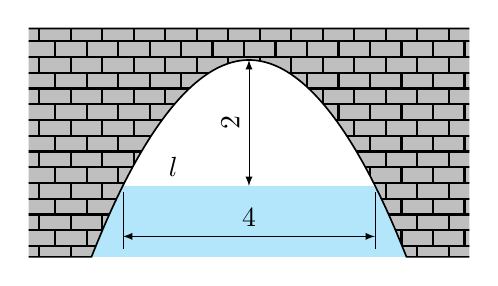
\begin{tikzpicture}[>=latex,scale=0.8]
  \fill[cyan!30!white](-3,-3.125)rectangle(3,-2);
  \fill[lightgray](-3.5,-3.125)--(-2.5,-3.125)parabola bend (0,0) (2.5,-3.125)--(3.5,-3.125)--(3.5,0.5)--(-3.5,0.5)--cycle;
  \fill[pattern=bricks](-3.5,-3.125)--(-2.5,-3.125)parabola bend (0,0) (2.5,-3.125)--(3.5,-3.125)--(3.5,0.5)--(-3.5,0.5)--cycle;
  \draw[semithick](-3.5,-3.125)--(-2.5,-3.125)parabola bend (0,0) (2.5,-3.125)--(3.5,-3.125)(3.5,0.5)--(-3.5,0.5);
  \draw[very thin] (-2,-2.1)--(-2,-3)(2,-2.1)--(2,-3);
  \draw[very thin,<->](0,-2)--(0,0)node[midway,sloped,above]{$2$};
  \draw[very thin,<->](-2,-2.8)--(2,-2.8)node[midway,above]{$4$};
  \node at (-1.2,-2)[above]{$l$};
\end{tikzpicture}
\end{document}